\section{Durchführung}
\label{sec:Durchführung}

\begin{figure}
    \centering
    \caption{Aufbau}
    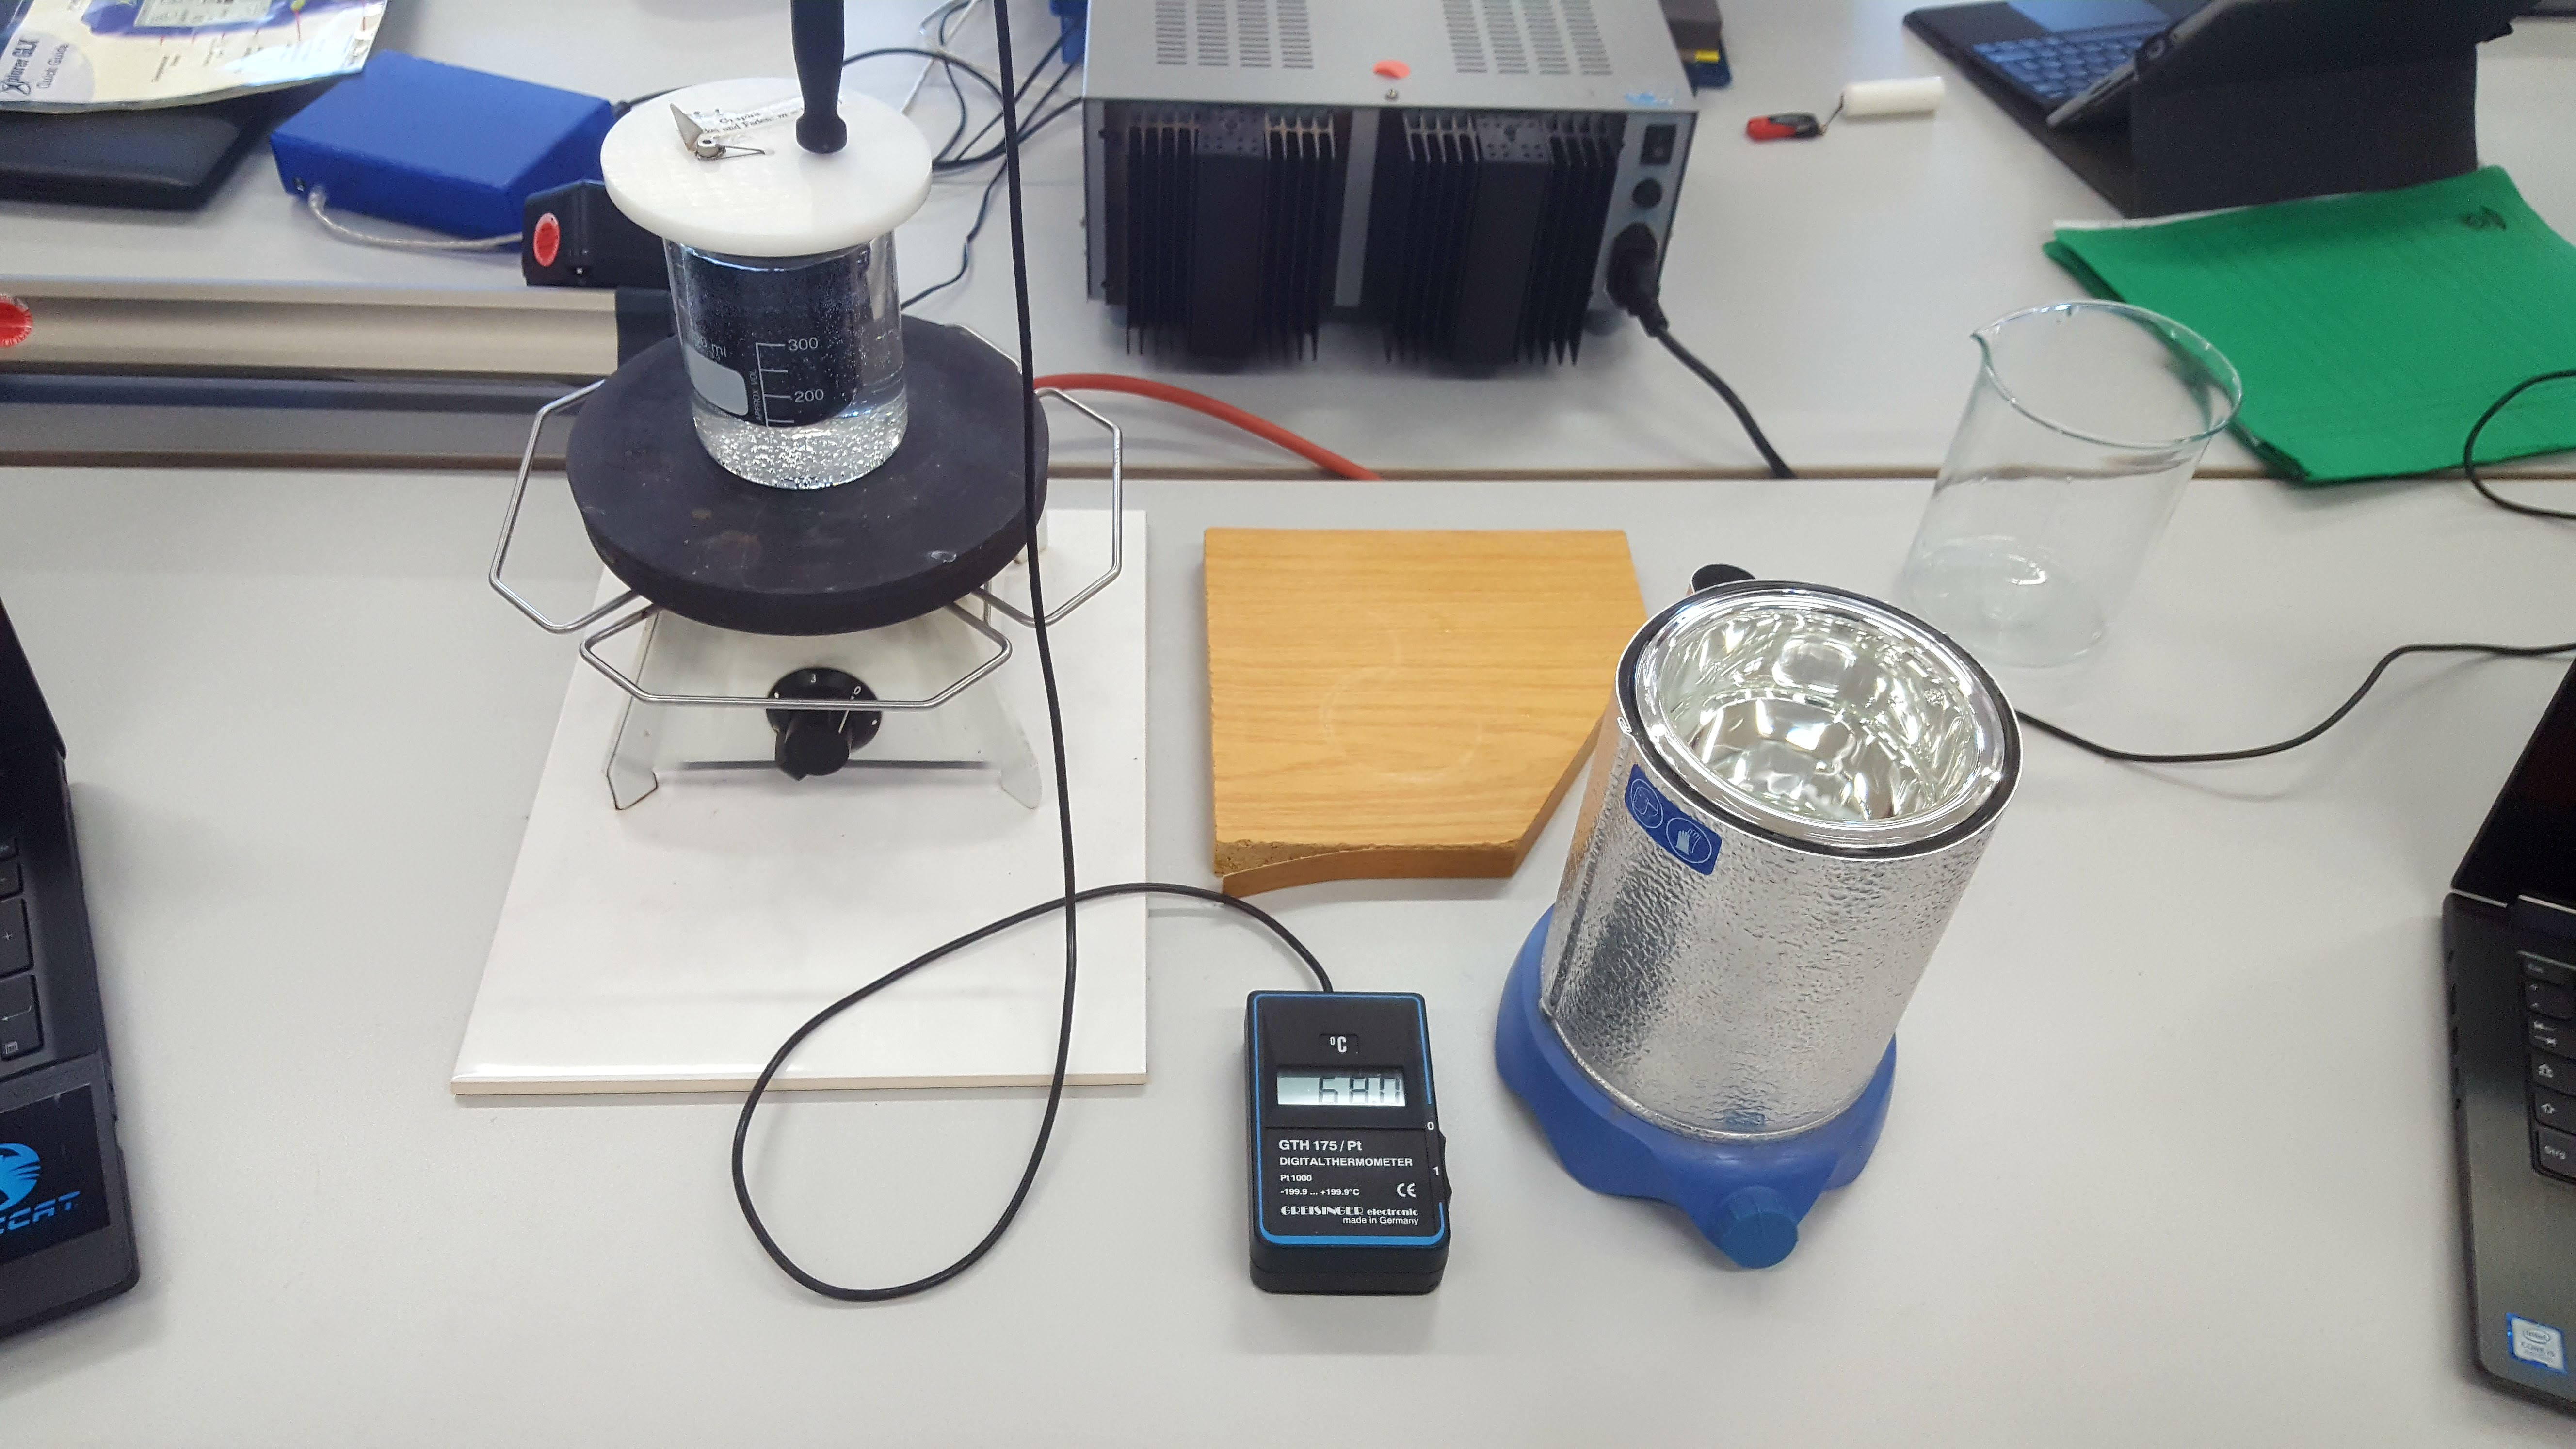
\includegraphics[height=6cm]{data/bild3.jpg}
\end{figure}

\subsection{Spezfische Wärmekapazitäten unterschiedlicher Materialien}

Der zu untersuchende Probekörper wird in ein Becherglas, welches mit Wasser gefüllt ist, gelegt. Dieses wird mit einer Heizplatte
bis auf etwa 80\si{\celsius} bis 90\si{\celsius} erhitzt. Die Temperatur wird mit einem Thermometer abgelesen. Nach dem Erhitzen wird der 
Probekörper aus dem heißen Wasser in ein Dewargefäßes gelegt, welches mit einer abgewogenen Menge Wasser gefüllt ist. Die Temperatur
des Wassers im Dewargefäß entspricht etwa der Raumtemperatur und wird immer vor dem Einsetzen des Probekörpers gemessen. Nachdem der
Probekörper in das Dewargefäß gelegt wird, wird der Verlauf der Wassertemperatur beobachtet und es wird nach etwa einer Minute,
wenn sich die Temperatur nicht mehr ändert, die
Mischtemperatur des Wassers notiert. Es sollte dabei nicht zu lange gewartet werden, da möglichst keine Wärme vom Dewargefäß an 
die Umgebung abgegeben werden sollte. 

Nach jeder Messung wird das Wasser im Dewargefäß ausgetauscht, um für jede erneute Durchführung die Bedingungen nicht zu variieren.

Die Messung wird mit drei unterschiedlichen Materialien, Kupfer, Zinn und Graphit durchgeführt. Für Kupfer und Zinn werden drei
Messungen gemacht, für Graphit nur eine.

\subsection{Wärmekapazität des Dewargefäßes}

Für die Bestimmung der Wärmekapazität des Dewargefäßes werden zwei möglichst gleiche, abgewogene Mengen Wasser unterschiedlicher
Temperaturen im Dewargefäß gemischt. Eine der Wassermengen wird auf der Heizplatte auf etwa 80\si{\celsius} erhitzt. Der andere
Teil des Wassers, dessen gemessene Temperatur ungefähr der Raumtemperatur entspricht, befindet sich im Dewargefäß. 
Das erhitzte Wasser wird dann in das Dewargefäß gefüllt und es wird, wie bei den Probekörpern auch, nach kurzer Zeit die 
Mischtemperatur gemessen. Beim erhitzen des Wassers muss besonders darauf geachtet werden, dass dieses nicht seinen Siedepunkt,
überschreitet, da damit Masse verloren ginge, was die Messwerte verfälschen würde.

